\section{Exploring Music Digital Libraries}

Musicological knowledge is spread between the lines of thousand of texts stored in hundreds of Music Libraries. Technology, and more recently semantic technologies, may play a key role in the way the information is retrieved. In this Section, an analysis of the evolution of Music Digital Libraries from a technological perspective is presented. Then, a methodology to exploit implicit knowledge present in collections of text documents is proposed. The described methodology is applied over a set of 16,707 artist biographies gathered from the New Grove Dictionary. 
Several insights are extracted from the data to illustrate the possibilities of the proposed methodology for musicologists.

\subsection{Evolution of Music Libraries}

Music Libraries can be classified according to their level of technology development. Following this criterion, a pyramid can be constructed, defining the different evolution states of a Music Library (see Figure~\ref{fig:musicology:pyramid}). The base of the pyramid represents traditional libraries, where items are physical, such as books, scores, manuscripts, slate records, etc. Items are often classified into catalogs and indexes. In last few decades, digitization of content has raised a new way of storing and making items available. They can be replicated, and even accessed online from anywhere in the world. Scores and books are scanned and the resulting images are stored in databases. Music can also be stored using digital audio formats. Thus, items can be consulted on a digital device (e.g. computer, smart phone, tablet). This has been the first great revolution for Music Libraries. Before that, musicologists had to be physically in the library to study texts or listen to audio. Nowadays, thanks to the efforts put into digitization and publication of content, musicologists and general public may have access to items everywhere.

Digitized items are generally stored in a database along with contextual information about them (e.g. title, author, date of publishing, etc.), which is generally called metadata. Metadata can be exploited by the search system of a Digital Library. Information retrieval techniques can be applied to Digital Libraries to navigate and search within the library. However, these kind of digitized items are not readable by the computer, so it is not possible to perform searches directly on the content of the item. Hence, there is a need of a further step in the evolution of Digital Libraries, transforming digitized items into machine-readable ones. To do so, items content must be transcribed into a proper format. Transcription can be done manually by humans, or automatically by a computer. Different techniques can be applied to perform this automatic transcription process. Scanned texts and scores can be automatically converted into machine-readable formats using optical character recognition (OCR) and optical music recognition (OMR) systems. Texts can be stored in txt, html or xml formats, and scores in midi or xml. 
Once the content is transcribed, the library search system may have access to the content itself. In the case of text documents, information retrieval techniques for searching documents can be applied on the whole content of the items, not only on the metadata. 

At this stage, Digital Libraries have increased significantly their ability to provide concrete answers to their users. However, the epistemic potential of the content is not being exploited yet. Computers are able to find patterns of words, but they do not understand the meaning of texts. Users can do simple text queries, but cannot ask complex questions. Let us illustrate it with an example. Imagine a Digital Library with thousands of biographies, scores and audio files from the Baroque period. A user wants to know the artists that were born in Italy and had worked in France, or the pieces with sonata form from German composers born in the second half of the 17th century. In their current state, Digital Libraries could not possibly provide an answer directly; it would be necessary to spend an important amount of time consulting different documents. Therefore, Digital Libraries should go a step further to make the content understandable by the computer, and provide the user with the tools to exploit this knowledge. One way to do so is by adding semantic annotations to the content. This annotation process can also be done either manually or automatically. Manual annotation requires a huge human effort, and most of the times it is infeasible. Therefore, automatic processes for semantic annotation are necessary to extract the knowledge behind the lines. A huge effort has been done in this direction in the Semantic Web and Natural Language Processing communities, developing tools and methodologies for Named Entity Recognition and Disambiguation, Relation Extraction and Information Extraction. 

Once library systems are able to understand all their content, the next step would be to become intelligent systems. At this stage, library systems would be able to perform their own reasoning processes by interconnecting knowledge from different documents and sources. They would be more a research partner than a mere search tool. They would be able to perform a complete research task from beginning to end and arrive to their own conclusions. Instead of search boxes, these library systems would display request boxes where musicologists can ask scientific questions. The web retrieval research community is already moving towards this direction. Music Digital Libraries should take advantage of these technological developments to improve their systems and advance towards a better understanding and dissemination of musical knowledge.

\begin{figure}[!ht]
	\centering
	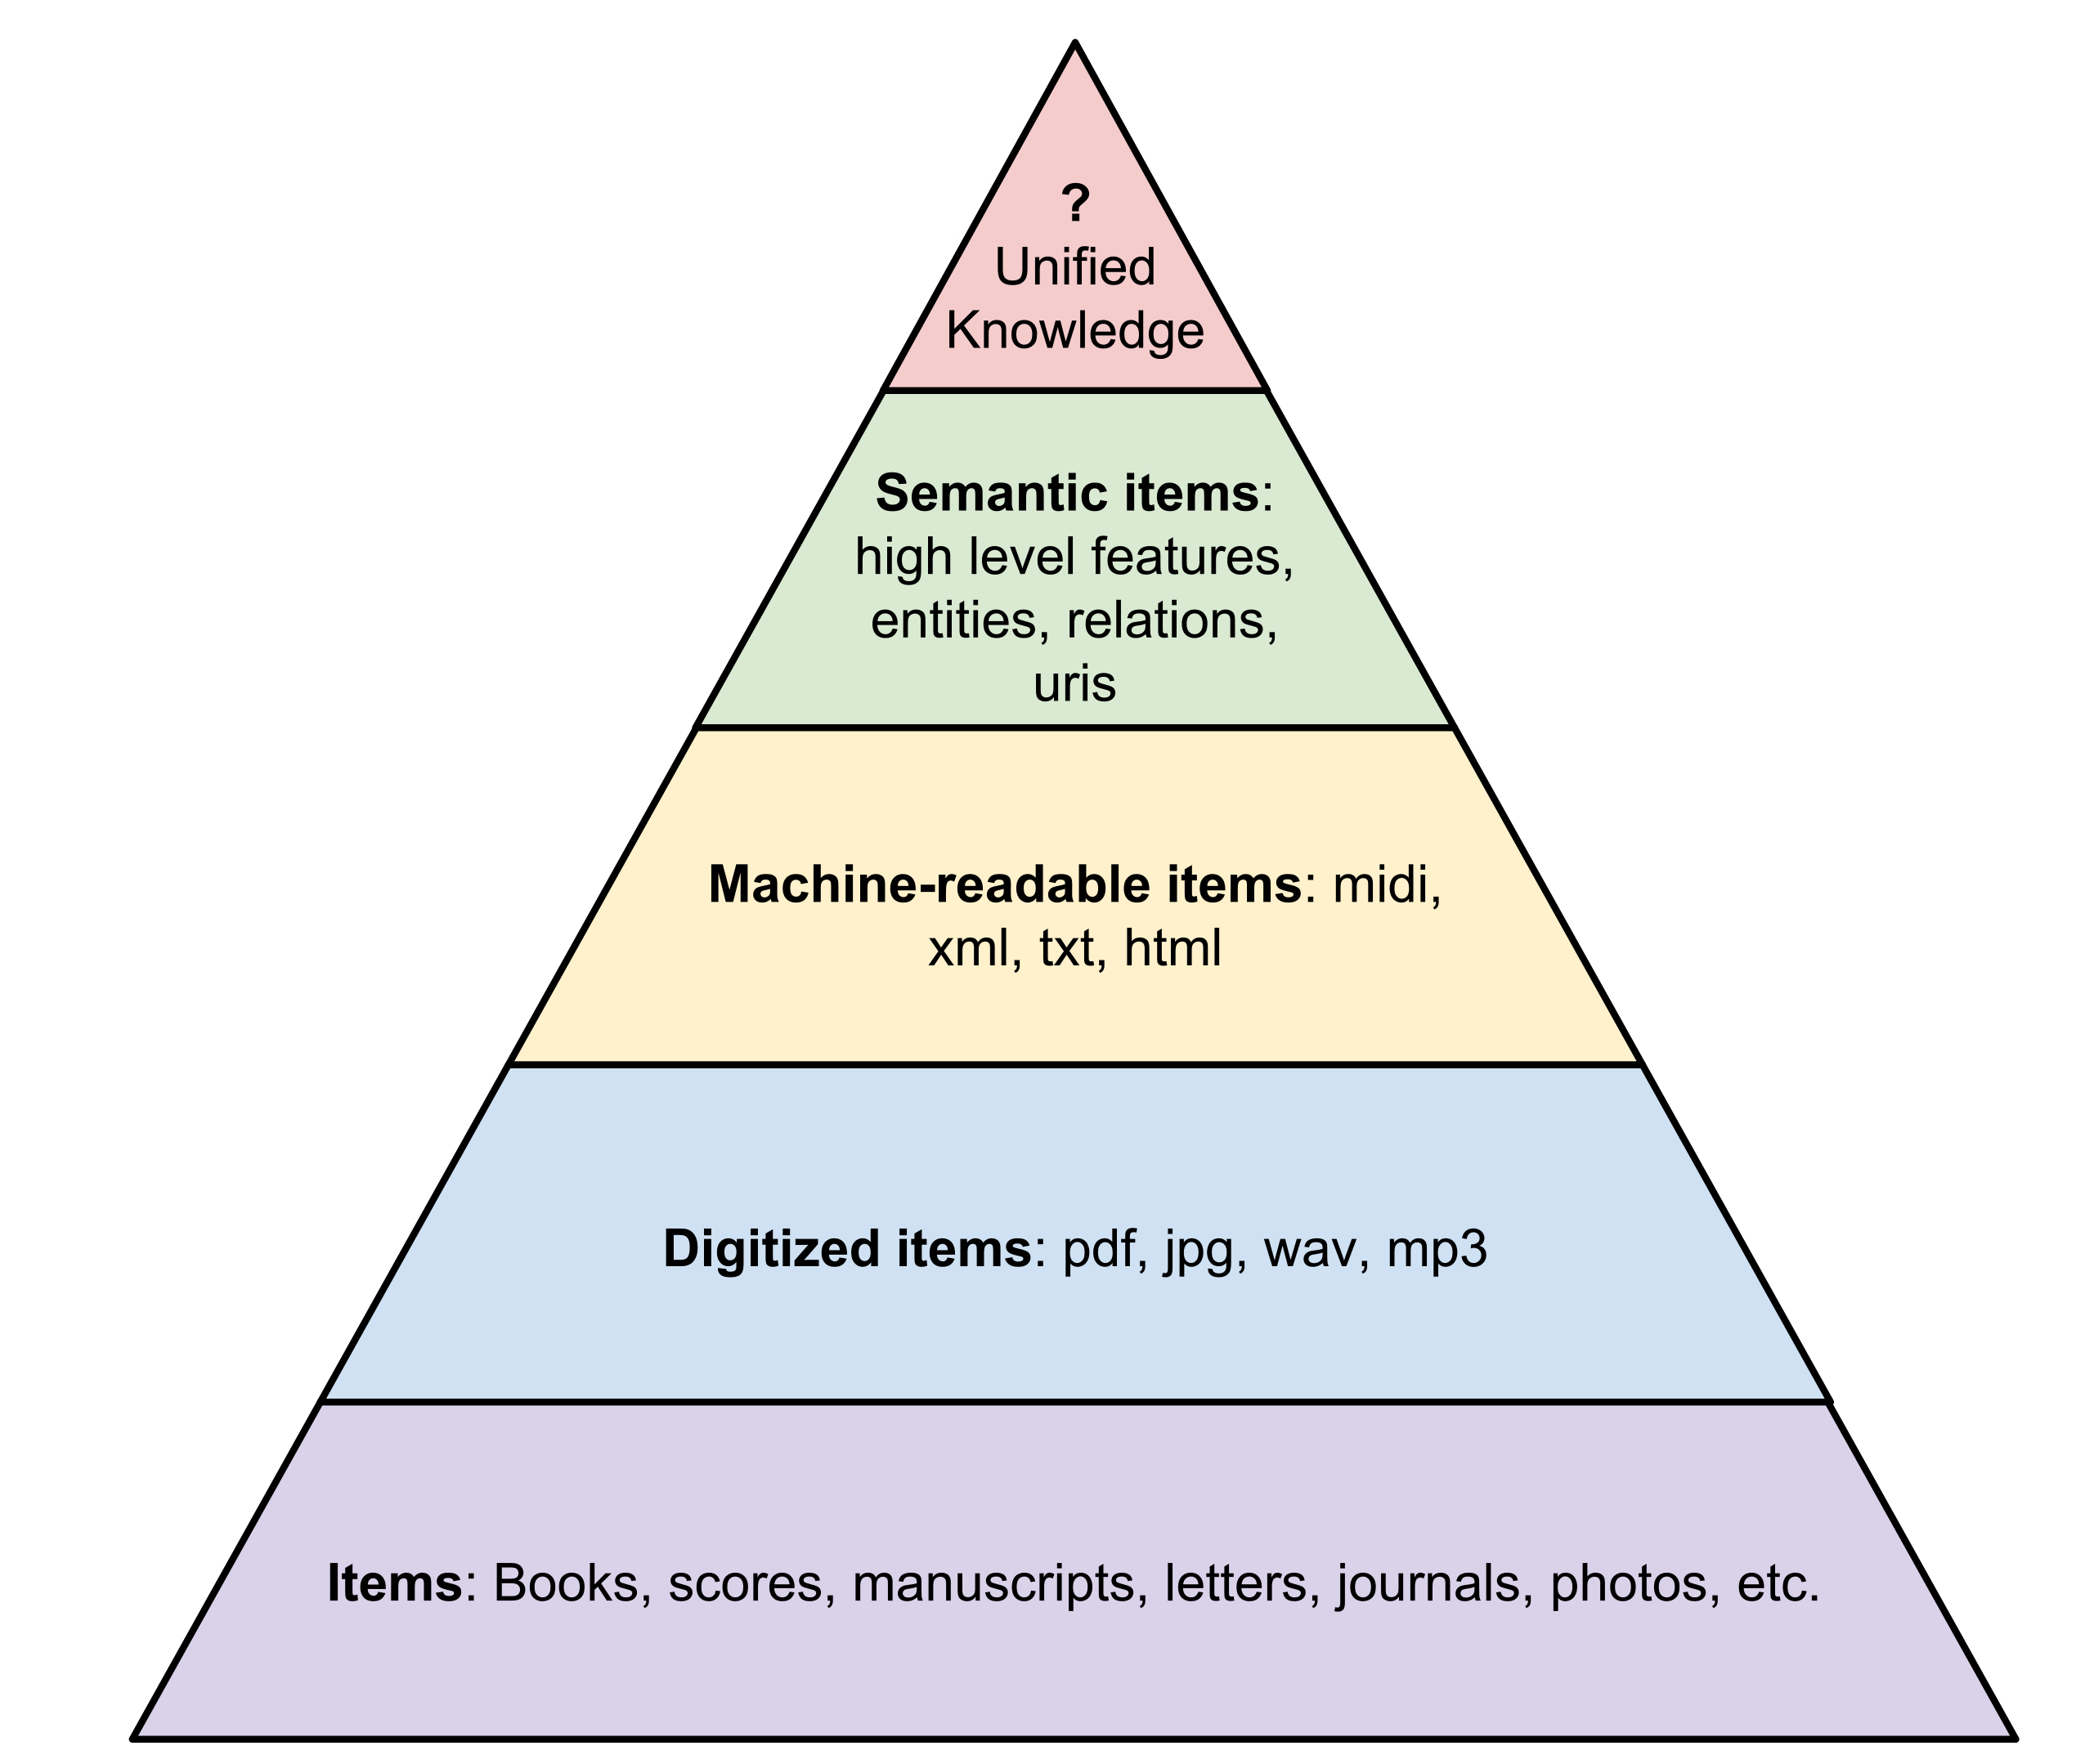
\includegraphics[width=8cm]{ch05_musicology_pics/evolution-dl.jpg}
	\caption{Pyramid of evolution states of a Music Library
	\label{fig:musicology:pyramid}}
\end{figure}


\subsection{Methodology}

This section defines a methodology to extract and exploit knowledge from documents in Music Digital Libraries (see Figure~\ref{fig:musicology:methodology-dl}). The idea is to gather the content and metadata from all the documents present in the library and then apply a process of semantic enrichment. This process consists in applying different processes of Information Extraction, such as Entity Linking and Relation Extraction. The goal is to build a Knowledge Base expressing the relations between entities present in the library. 
An item of the library corresponds to an entity in the KB. In addition, a process of Entity Linking is applied to the content of every item, and every entity mention detected on it is also added to the KB. Entities can be related by different kind of relations. These relations can be gathered from metadata, or extracted from the text itself by applying Relation Extraction techniques. Moreover, the KB can be related to, or linked to other existing KBs, thus leveraging the power of the Linked Open Data (LOD) initiative. 
Once the KB is built, a graph representation of the data can be easily constructed. This representation can be expressed as a simple graph, or as an RDF graph. We call this representation a Knowledge Graph. The Knowledge Graph can be exploited in different applications, such as artist relevance, artist similarity, music recommendation, or information visualization (See Chapter~\ref{}).

\begin{figure}[!ht]
	\centering
	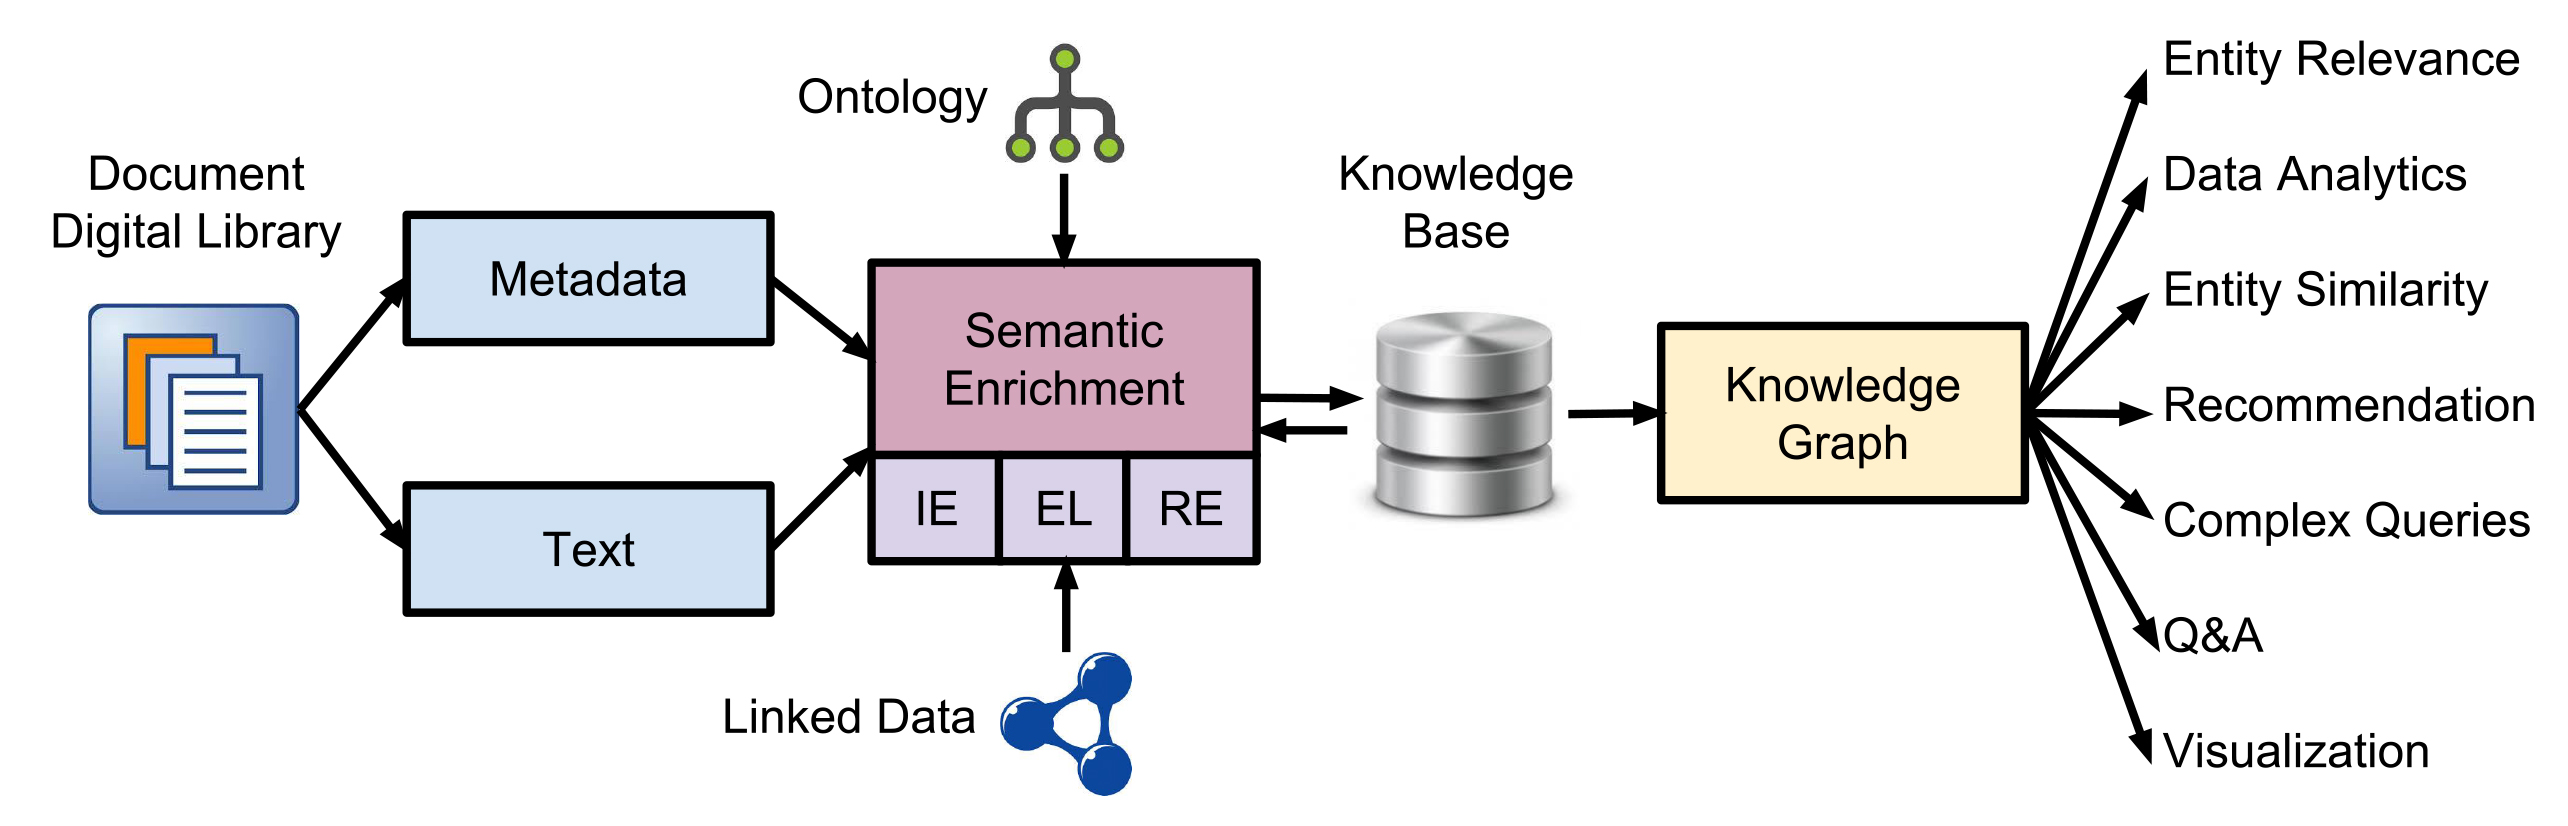
\includegraphics[width=8cm]{ch05_musicology_pics/methodology-dl.jpg}
	\caption{Methodology
	\label{fig:musicology:methodology-dl}}
\end{figure}

\subsection{Experiments}

In this Section, the proposed methodology is applied to a Music Digital Library. The objective here is to illustrate the possibilities of the methodology for discovering new knowledge, and help musicologists when using a Digital Library.

\subsubsection{Dataset: The New Grove}

The Grove Dictionary of Music and Musicians is an encyclopedic dictionary, and one of the largest works of reference in Western music. George Grove first published it in the last quarter of the 19th century. In 1980 a new version called The New Grove  was released with 20 volumes, consisting of 22,500 articles and more than 16k biographies. The complete text of the second edition of The New Grove is available in machine-readable format on the online service Grove Music Online .
We automatically gathered the first paragraph of every biography classified in the section People in history in the Grove Music Online. These biographies are related to artists from different periods of the history of music, from Pre-medieval time to contemporary. We obtained a total of 16,707 biographies.

\subsubsection{Information Extraction}

To create our Knowledge Base, we followed a process similar to the one explained in Section~\ref{}. This time, we used two different Entity Linking procedures.
The first consisted in building a gazetteer, a list of artist subjects in the library, and performing a simple string matching on the biography texts, looking for entity mentions. This way, we detected most of the auto references of entities within the library. The second procedure dealt with the detection of other types of entities, such as Educational Institutions, Music Genres, Places and Concert Venues. To detect these entities, we used TagMe, a state-of-the-art Entity Linking tool. 
We used the type information provided by TagMe to filter out entity mentions, keeping only those of the desired types. After the Entity Linking process we created a graph in the same way is explained in Section~\ref{}.

By observing the biographical texts, we detected some common structures. For example, at the beginning of every biography there is a sentence between parentheses with information about the place and date of birth and death. In addition, the second sentence of the biography is always describing the role of the biography subject. Therefore, we applied a process of Information Extraction to obtain the roles, and the place and year of birth and death from every biography similar to the one described in Section~\ref{}. We obtained birth information for 14,355 subjects, and death information for 10,741. As for the roles, we collected 434 different roles. The most represented roles in the dataset are shown in Table 1. 

Role	Amount
composer	2618
teacher	1065
conductor	968
pianist	704
organist	676
singer	404
violinist	285
…	
musicologist	144
critic	133

Table 1: Most representative roles in the dataset


\subsubsection{Data Analytics}

We built a histogram with the amount of births per decade (see Figure~\ref{fig:musicology:hist-births}). In this histogram the distribution of artist births along the history is represented. We easily observe that there is a peak of births on the second half of the 16th century and on the second half of 18th century. Note that the scope of this research is not to extract musicological conclusions, but to show in which way semantic technology may help the musicologist. 
We also counted the number of births and deaths by country. Table 2 shows the number of births and deaths and the perceptual difference between both values for the five countries with more births. We observe that United States and Italy have a negative percentage. This means that there is a migratory tendency of their artists. However, France has a positive value, so it has absorbed artists from abroad. The same count for the five cities with more births is shown in Table 3. All these cities have an absorbing tendency. Perhaps the case of Paris draws more attention with an increase of 137%. 

\begin{figure}[!ht]
	\centering
	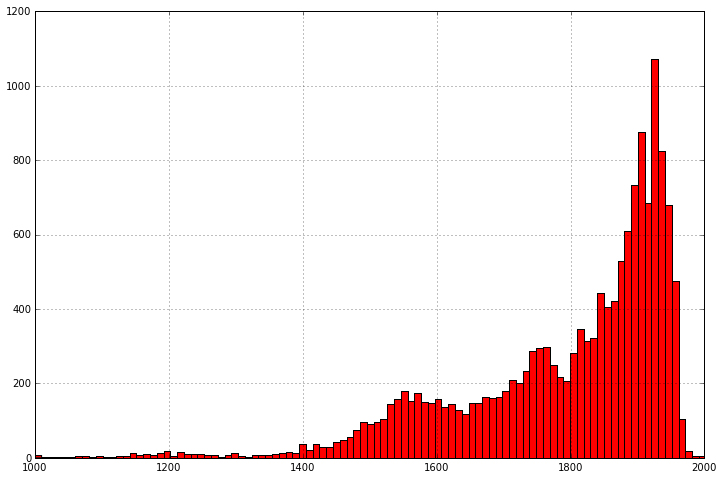
\includegraphics[width=8cm]{ch05_musicology_pics/histogram-births.jpg}
	\caption{Histogram of births by decade
	\label{fig:musicology:hist-births}}
\end{figure}

Country	Births	Deaths	Difference
United States	2317	2094	-10%
Italy	1616	1279	-21%
Germany	1270	1292	2%
France	991	1058	7%
United Kingdom	882	877	-1%

Table 2: Number of births and deaths by country


City	Births	Deaths	Difference
London	322	507	57%
Paris	304	720	137%
New York	266	501	88%
Vienna	177	292	65%
Rome	159	256	61%

Table 3: Number of births and deaths by city